%%%%%%%%%%%%%%%%%%%%%%%%%%%%% Define Article %%%%%%%%%%%%%%%%%%%%%%%%%%%%%%%%%%
\documentclass{article}
%%%%%%%%%%%%%%%%%%%%%%%%%%%%%%%%%%%%%%%%%%%%%%%%%%%%%%%%%%%%%%%%%%%%%%%%%%%%%%%

%%%%%%%%%%%%%%%%%%%%%%%%%%%%% Using Packages %%%%%%%%%%%%%%%%%%%%%%%%%%%%%%%%%%
\usepackage{geometry}
\usepackage{graphicx}
\usepackage{amssymb}
\usepackage{amsmath}
\usepackage{amsthm}
\usepackage{empheq}
\usepackage{mdframed}
\usepackage{booktabs}
\usepackage{lipsum}
\usepackage{graphicx}
\usepackage{color}
\usepackage{psfrag}
\usepackage{pgfplots}
\usepackage{bm}


%%%%%%%%%%%%%%%%%%%%%%%%%%%%%%%%%%%%%%%%%%%%%%%%%%%%%%%%%%%%%%%%%%%%%%%%%%%%%%%

% Other Settings

%%%%%%%%%%%%%%%%%%%%%%%%%% Page Setting %%%%%%%%%%%%%%%%%%%%%%%%%%%%%%%%%%%%%%%
\geometry{a4paper}

%%%%%%%%%%%%%%%%%%%%%%%%%% Define some useful colors %%%%%%%%%%%%%%%%%%%%%%%%%%
\definecolor{ocre}{RGB}{243,102,25}
\definecolor{mygray}{RGB}{243,243,244}
\definecolor{deepGreen}{RGB}{26,111,0}
\definecolor{shallowGreen}{RGB}{235,255,255}
\definecolor{deepBlue}{RGB}{61,124,222}
\definecolor{shallowBlue}{RGB}{235,249,255}
%%%%%%%%%%%%%%%%%%%%%%%%%%%%%%%%%%%%%%%%%%%%%%%%%%%%%%%%%%%%%%%%%%%%%%%%%%%%%%%

%%%%%%%%%%%%%%%%%%%%%%%%%% Define an orangebox command %%%%%%%%%%%%%%%%%%%%%%%%
\newcommand\orangebox[1]{\fcolorbox{ocre}{mygray}{\hspace{1em}#1\hspace{1em}}}
%%%%%%%%%%%%%%%%%%%%%%%%%%%%%%%%%%%%%%%%%%%%%%%%%%%%%%%%%%%%%%%%%%%%%%%%%%%%%%%

%%%%%%%%%%%%%%%%%%%%%%%%%%%% English Environments %%%%%%%%%%%%%%%%%%%%%%%%%%%%%
\newtheoremstyle{mytheoremstyle}{3pt}{3pt}{\normalfont}{0cm}{\rmfamily\bfseries}{}{1em}{{\color{black}\thmname{#1}~\thmnumber{#2}}\thmnote{\,--\,#3}}
\newtheoremstyle{myproblemstyle}{3pt}{3pt}{\normalfont}{0cm}{\rmfamily\bfseries}{}{1em}{{\color{black}\thmname{#1}~\thmnumber{#2}}\thmnote{\,--\,#3}}
\theoremstyle{mytheoremstyle}
\newmdtheoremenv[linewidth=1pt,backgroundcolor=shallowGreen,linecolor=deepGreen,leftmargin=0pt,innerleftmargin=20pt,innerrightmargin=20pt,]{theorem}{Theorem}[section]
\theoremstyle{mytheoremstyle}
\newmdtheoremenv[linewidth=1pt,backgroundcolor=shallowBlue,linecolor=deepBlue,leftmargin=0pt,innerleftmargin=20pt,innerrightmargin=20pt,]{definition}{Definition}[section]
\theoremstyle{myproblemstyle}
\newmdtheoremenv[linecolor=black,leftmargin=0pt,innerleftmargin=10pt,innerrightmargin=10pt,]{problem}{Problem}[section]
%%%%%%%%%%%%%%%%%%%%%%%%%%%%%%%%%%%%%%%%%%%%%%%%%%%%%%%%%%%%%%%%%%%%%%%%%%%%%%%

%%%%%%%%%%%%%%%%%%%%%%%%%%%%%%% Plotting Settings %%%%%%%%%%%%%%%%%%%%%%%%%%%%%
\usepgfplotslibrary{colorbrewer}
\pgfplotsset{width=8cm,compat=1.9}
\usetikzlibrary{shapes}
%%%%%%%%%%%%%%%%%%%%%%%%%%%%%%%%%%%%%%%%%%%%%%%%%%%%%%%%%%%%%%%%%%%%%%%%%%%%%%%

\title{Title}
\author{Aaditya Salgarkar}
%%%%%%%%%%%%%%%%%%%%%%%%%%%%%%%%%%%%%%%%%%%%%%%%%%%%%%%%%%%%%%%%%%%%%%%%%%%%%%%

\begin{document}
\maketitle
\begin{figure}[htbp]
    \centering

    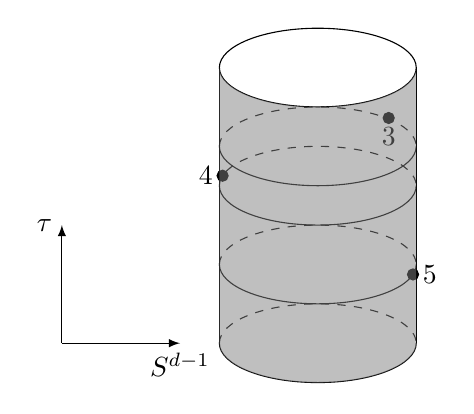
\begin{tikzpicture}
        \draw (0,0) ellipse (1.25 and 0.5);
        \draw (-1.25,0) -- (-1.25,-3.5);
        \draw (1.25,-3.5) -- (1.25,0);
        \filldraw[black ] (1.25 * 0.72, 0.5 *0.72-1 ) circle (2pt);

        \node[below] at(1.25 * 0.72, 0.5 *0.72 -1 ){$3$};
        \filldraw[black ] (1.25 * -0.967251, 0.5 *0.253823 -1.5 ) circle (2pt);
        \node[left] at (-1.25 * 0.967251, 0.5 *0.253823 -1.5 ){$4$};

        \filldraw[black ] (1.25 * 0.967251, -0.5 *0.253823 -2.5 ) circle (2pt);
        \node[right] at (1.25 * 0.967251, -0.5 *0.253823 -2.5 ){$5$};
        \draw[->,-latex] (-3.25,-3.5) -- (-3.25,-2);
        \draw[->,-latex] (-3.25,-3.5) -- ( -1.75 ,-3.5);

        \node[left] at (-3.25,-2) {$ \tau $};
        \node[below] at (-1.75, -3.5) {$ S^{d-1} $};

        \draw (-1.25,-1.5) arc (180:360:1.25 and 0.5);
        \draw [dashed] (-1.25,-1.5) arc (180:360:1.25 and -0.5);
        \draw (-1.25,-3.5) arc (180:360:1.25 and 0.5);
        \draw [dashed] (-1.25,-3.5) arc (180:360:1.25 and -0.5);

        \draw (-1.25,-1.0) arc (180:360:1.25 and 0.5);
        \draw [dashed] (-1.25,-1.0) arc (180:360:1.25 and -0.5);

        \draw (-1.25,-2.5) arc (180:360:1.25 and 0.5);
        \draw [dashed] (-1.25,-2.5) arc (180:360:1.25 and -0.5);
        \fill [gray,opacity=0.5] (-1.25,0) -- (-1.25,-3.5) arc (180:360:1.25 and 0.5) -- (1.25,0) arc (0:180:1.25 and -0.5);

    \end{tikzpicture}
    \caption{Position of points on the Euclidean cylinder. Two points $ 1 $ and $ 2 $, are at $ \tau =  -\infty $ and $ \tau = \infty $.}
    \label{fig:euclidean_cylinder}
\end{figure}
\end{document}